
\style{mb}


\section{Dé à 6 faces avec \mb}

\subsection{Description}

\subsubsection{Objectif}

\begin{formule}
Le but de ce projet est de simuler une expérience aléatoire de lancer de dé à 6 faces avec une carte \mb.

Toujours à partir d’une situation simple idéale, le programme peut être étoffé au gré des besoins. Il s'agit de prolonger les quelques notions utilisées pour l'activité pile ou face, notamment lorsqu'il faudra tester les différentes issues et proposer une sortie en conséquence.
\end{formule}

\subsubsection{Intérêt}
L'intérêt de cette activité n'est pas seulement de se départir des bruits des dés qui roulent dans la classe; l'usage du \mb est ici très pertinent, tant pour les probabilités que pour la programmation.
\begin{description}
    \item [Simplicité de la situation.] La situation est très simple à expliquer et les élèves comprennent le but à atteindre. L'absence de difficulté mathématique rend cette situation particulièrement simple à mettre en œuvre.
    \item [Motivation des élèves.] L'envie de programmer un objet connecté est grande pour les élèves. Cette façon de programmer, \emph{utile, concrète et appliquée}, leur correspond parfaitement.
    \item [De nombreuses solutions/améliorations possibles.] Comme pour bien des projets, il y a plusieurs façons d'arriver à la solution; mais par rapport à l'activité \emph{Pile ou Face} il y aussi plus de possibilité de faire des erreurs de programmation.
    \item [Travail mathématique sur la modélisation.] La modélisation d'un dé non truqué est évidente, et n'apporte pas de difficulté majeure. Par contre l'intérêt majeur du \mb est d'offrir la possibilité de truquer le dé. On a alors une situation beaucoup plus riche, tant dans la modélisation que dans les usages du modèle obtenu.
\end{description}


\subsubsection{Matériel}
\begin{itemize}
    \item 1 $\times$ \matosMb \emph{(facultatif car le simulateur peut suffire)}
    \item 1 $\times$ accès internet : IDE programmation par bloc \url{http://makecode.microbit.org/}
\end{itemize}


%
% activité de niveau 1
%
\newpage
\subsection{Niveau simple}
\subsubsection{Activité élève}

% commande perso \CARTOUCHE
%   5 paramètres : 
%       * durée
%       * public
%       * travail en maths
%       * travail en sciences
%       * travail en algo
\cartouche{0,25 h}{2de}{expérience aléatoire}{}{affichage ; événement.}

\begin{eleve}

\begin{wrapfigure}[4]{r}{3.5cm}
	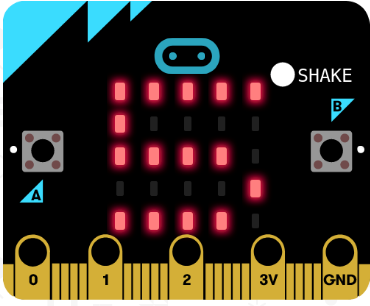
\includegraphics[width=\linewidth]{res/mbDe6FacesN1.png}
\end{wrapfigure}

\texttt{\textsc{Mission} Utilise \mb~pour simuler un \emph{dé à 6 faces} !}


En t'aidant des blocs ci-dessous, programme \mb~pour : 
\begin{enumerate}
    \item programmer un événement lorsque l'appareil est secoué;
    \item afficher \emph{un nombre entier aléatoire} entre \texttt{1} et \texttt{6}.
\end{enumerate}
~\\
\centerline{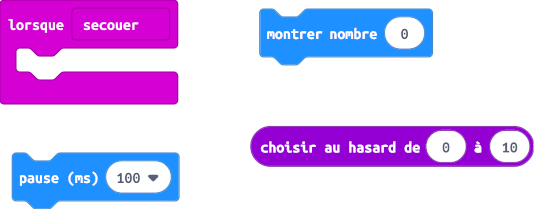
\includegraphics[width=0.6\textwidth]{res/mbDe6FacesN1blocs.png}}

\end{eleve}


\subsubsection{Notes pour l'enseignant}

Ce premier niveau aucun niveau de difficulté, on pourrait dire que son intérêt se limite à poser la problématique.

\begin{minipage}[t]{0.5\linewidth}
    \begin{methode}
    ~\\Pour résoudre ce problème, il suffit de programmer les instructions de la façon suivante :
    
    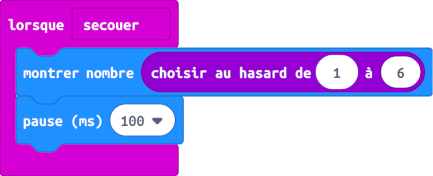
\includegraphics[width=0.4\linewidth]{res/mbDe6FacesN1proposition.png}
    \end{methode}
\end{minipage}
\hfill
\begin{minipage}[t]{0.5\linewidth}
    \begin{remarque}
    ~\\Plus d'informations sur la page de l'activité :\\ \url{https://microbit.readthedocs.io/fr/latest/decouverte/de6faces-bloc1.html}
    \end{remarque}
\end{minipage}






%
% activité de niveau 2
%
\newpage
\subsection{Niveau intermédiaire}
\subsubsection{Activité élève}

% commande perso \CARTOUCHE
%   5 paramètres : 
%       * durée
%       * public
%       * travail en maths
%       * travail en sciences
%       * travail en algo
\cartouche{0,5 h}{2de}{expérience aléatoire}{}{affichage ; événement ; condition}


\begin{eleve}
	
	
\begin{wrapfigure}[7]{r}{4cm}
	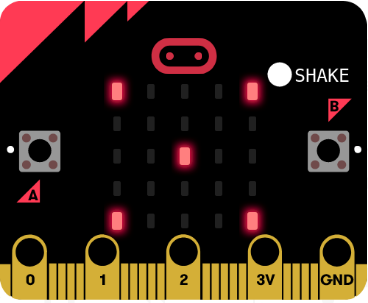
\includegraphics[width=\linewidth]{res/mbDe6FacesN2.png}
\end{wrapfigure}

Utilise \mb~pour simuler un \emph{dé à 6 faces} !

En t'aidant des blocs ci-dessous, programme \mb~pour : 
\begin{enumerate}
    \item programmer un événement lorsque l'appareil est secoué;
    \item afficher \emph{une face de dé} selon le résultat d'un tirage aléatoire.
\end{enumerate}
Attention tous les blocs ne sont pas représentés et certains blocs doivent être modifiés.

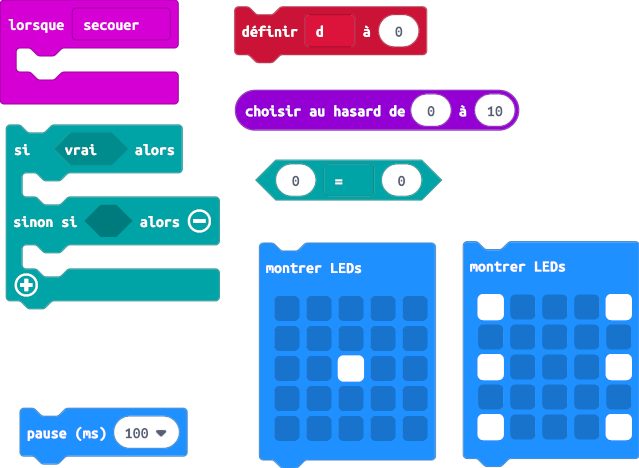
\includegraphics[width=0.6\textwidth]{res/mbDe6FacesN2blocs.png}

\end{eleve}

\newpage
\subsubsection{Notes pour l'enseignant}

Pour arriver au résultat escompté il est nécessaire d'utiliser une variable, ainsi qu'une suite d'instruction si/sinon si/sinon. Si l'usage d'une variable n'apparaît pas forcément évident pour les élèves, on peut les laisser programmer sans pour qu'il puisse ainsi constater le bug produit.
Il est aussi intéressant de faire remarquer aux élèves que le nombre issue du tirage aléatoire n'a pas forcément à être celui symbolisé par sortie sur l'écran de DEL.


\begin{minipage}[t]{0.5\linewidth}
    \begin{methode}~\\
    Pour résoudre ce problème, il suffit de programmer les instructions de la façon suivante (seules les sorties correspondant à 1 et à 6 ont été incluses, pour raison de place) :
    
    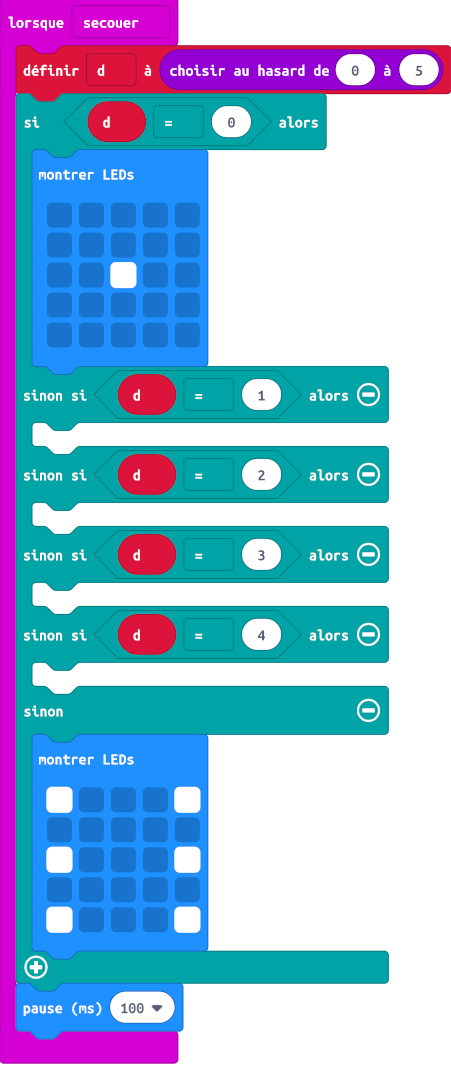
\includegraphics[width=0.85\linewidth]{res/mbDe6FacesN2propos.png}
    \end{methode}
\end{minipage}
\hfill
\begin{minipage}[t]{0.5\linewidth}
    \begin{remarque}~\\
    Il est très simple en partant de cette situation d'envoyer les résultats par radio ver un \mb qui centraliserait alors les issues de l'ensemble des tirages. Pour cela il suffit d'ajouter le bloc "envoyer le nombre" qui se trouve dans la catégorie "Radio".
    
    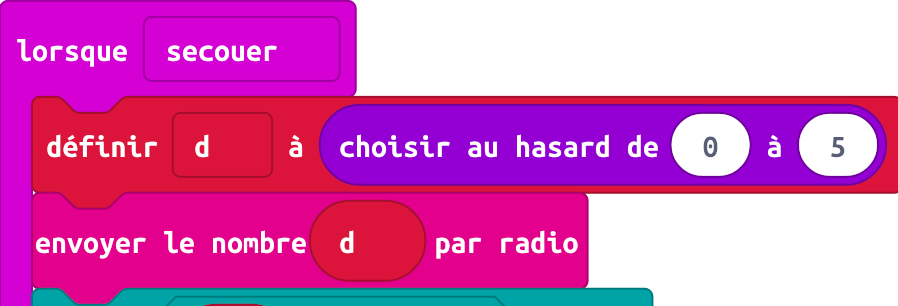
\includegraphics[width=\linewidth]{res/mbDe6FacesN2radio.png}
    
    Plus d'informations sur la page de l'activité :\\ \url{https://microbit.readthedocs.io/fr/latest/decouverte/de6faces-bloc2.html}
    \end{remarque}
\end{minipage}